% hw4.tex

% !TEX program = xelatex
%%%%%%%%%%%%%%%%%%%%
% see http://mirrors.concertpass.com/tex-archive/macros/latex/contrib/tufte-latex/sample-handout.pdf
% for how to use tufte-handout
\documentclass[a4paper, justified]{tufte-handout}

% hw-preamble.tex

% geometry for A4 paper
% See https://tex.stackexchange.com/a/119912/23098
\geometry{
  left=20.0mm,
  top=20.0mm,
  bottom=20.0mm,
  textwidth=130mm, % main text block
  marginparsep=5.0mm, % gutter between main text block and margin notes
  marginparwidth=50.0mm % width of margin notes
}

% for colors
\usepackage{xcolor} % usage: \color{red}{text}
% predefined colors
\newcommand{\red}[1]{\textcolor{red}{#1}} % usage: \red{text}
\newcommand{\blue}[1]{\textcolor{blue}{#1}}
\newcommand{\teal}[1]{\textcolor{teal}{#1}}

\usepackage{todonotes}

% heading
\usepackage{sectsty}
\setcounter{secnumdepth}{2}
\allsectionsfont{\centering\huge\rmfamily}

% for Chinese
\usepackage{xeCJK}
\usepackage{zhnumber}
\setCJKmainfont[BoldFont=FandolSong-Bold.otf]{FandolSong-Regular.otf}

% for fonts
\usepackage{fontspec}
\newcommand{\song}{\CJKfamily{song}}
\newcommand{\kai}{\CJKfamily{kai}}

% To fix the ``MakeTextLowerCase'' bug:
% See https://github.com/Tufte-LaTeX/tufte-latex/issues/64#issuecomment-78572017
% Set up the spacing using fontspec features
\renewcommand\allcapsspacing[1]{{\addfontfeature{LetterSpace=15}#1}}
\renewcommand\smallcapsspacing[1]{{\addfontfeature{LetterSpace=10}#1}}

% for url
\usepackage{hyperref}
\hypersetup{colorlinks = true,
  linkcolor = teal,
  urlcolor  = teal,
  citecolor = blue,
  anchorcolor = blue}

\newcommand{\me}[4]{
    \author{
      {\bfseries 姓名:}\underline{#1}\hspace{2em}
      {\bfseries 学号:}\underline{#2}\hspace{2em}\\[10pt]
      {\bfseries 评分:}\underline{#3\hspace{3em}}\hspace{2em}
      {\bfseries 评阅:}\underline{#4\hspace{3em}}
  }
}

% Please ALWAYS Keep This.
\newcommand{\noplagiarism}{
  \begin{center}
    \fbox{\begin{tabular}{@{}c@{}}
      请独立完成作业,不得抄袭。\\
      若得到他人帮助, 请致谢。\\
      若参考了其它资料,请给出引用。\\
      鼓励讨论,但需独立书写解题过程。
    \end{tabular}}
  \end{center}
}

% \newcommand{\goal}[1]{
%   \begin{center}{\fcolorbox{blue}{yellow!60}{\parbox{0.50\textwidth}{\large
%     \begin{itemize}
%       \item 体会``思维的乐趣''
%       \item 初步了解递归与数学归纳法
%       \item 初步接触算法概念与问题下界概念
%     \end{itemize}}}}
%   \end{center}
% }

% Each hw consists of four parts:
\newcommand{\beginrequired}{\hspace{5em}\section{作业 (必做部分)}}
\newcommand{\beginoptional}{\section{作业 (选做部分)}}
\newcommand{\beginot}{\section{Open Topics}}
\newcommand{\begincorrection}{\section{订正}}
\newcommand{\beginfb}{\section{反馈}}

% for math
\usepackage{amsmath, mathtools, amsfonts, amssymb}
\newcommand{\set}[1]{\{#1\}}

% define theorem-like environments
\usepackage[amsmath, thmmarks]{ntheorem}

\theoremstyle{break}
\theorempreskip{2.0\topsep}
\theorembodyfont{\song}
\theoremseparator{}
\newtheorem{problem}{题目}[subsection]
\renewcommand{\theproblem}{\arabic{problem}}
\newtheorem{ot}{Open Topics}

\theorempreskip{3.0\topsep}
\theoremheaderfont{\kai\bfseries}
\theoremseparator{:}
\theorempostwork{\bigskip\hrule}
\newtheorem*{solution}{解答}
\theorempostwork{\bigskip\hrule}
\newtheorem*{revision}{订正}

\theoremstyle{plain}
\newtheorem*{cause}{错因分析}
\newtheorem*{remark}{注}

\theoremstyle{break}
\theorempostwork{\bigskip\hrule}
\theoremsymbol{\ensuremath{\Box}}
\newtheorem*{proof}{证明}

% \newcommand{\ot}{\blue{\bf [OT]}}

% for figs
\renewcommand\figurename{图}
\renewcommand\tablename{表}

% for fig without caption: #1: width/size; #2: fig file
\newcommand{\fig}[2]{
  \begin{figure}[htbp]
    \centering
    \includegraphics[#1]{#2}
  \end{figure}
}
% for fig with caption: #1: width/size; #2: fig file; #3: caption
\newcommand{\figcap}[3]{
  \begin{figure}[htbp]
    \centering
    \includegraphics[#1]{#2}
    \caption{#3}
  \end{figure}
}
% for fig with both caption and label: #1: width/size; #2: fig file; #3: caption; #4: label
\newcommand{\figcaplbl}[4]{
  \begin{figure}[htbp]
    \centering
    \includegraphics[#1]{#2}
    \caption{#3}
    \label{#4}
  \end{figure}
}
% for margin fig without caption: #1: width/size; #2: fig file
\newcommand{\mfig}[2]{
  \begin{marginfigure}
    \centering
    \includegraphics[#1]{#2}
  \end{marginfigure}
}
% for margin fig with caption: #1: width/size; #2: fig file; #3: caption
\newcommand{\mfigcap}[3]{
  \begin{marginfigure}
    \centering
    \includegraphics[#1]{#2}
    \caption{#3}
  \end{marginfigure}
}

\usepackage{fancyvrb}

% for algorithms
\usepackage[]{algorithm}
\usepackage[]{algpseudocode} % noend
% See [Adjust the indentation whithin the algorithmicx-package when a line is broken](https://tex.stackexchange.com/a/68540/23098)
\newcommand{\algparbox}[1]{\parbox[t]{\dimexpr\linewidth-\algorithmicindent}{#1\strut}}
\newcommand{\hStatex}[0]{\vspace{5pt}}
\makeatletter
\newlength{\trianglerightwidth}
\settowidth{\trianglerightwidth}{$\triangleright$~}
\algnewcommand{\LineComment}[1]{\Statex \hskip\ALG@thistlm \(\triangleright\) #1}
\algnewcommand{\LineCommentCont}[1]{\Statex \hskip\ALG@thistlm%
  \parbox[t]{\dimexpr\linewidth-\ALG@thistlm}{\hangindent=\trianglerightwidth \hangafter=1 \strut$\triangleright$ #1\strut}}
\makeatother

% for footnote/marginnote
% see https://tex.stackexchange.com/a/133265/23098
\usepackage{tikz}
\newcommand{\circled}[1]{%
  \tikz[baseline=(char.base)]
  \node [draw, circle, inner sep = 0.5pt, font = \tiny, minimum size = 8pt] (char) {#1};
}
\renewcommand\thefootnote{\protect\circled{\arabic{footnote}}}

\newcommand{\score}[1]{{\bf [#1 分]}}

\newcommand{\rel}[1]{\xrightarrow{#1}}
\newcommand{\dstar}{\xRightarrow[]{\ast}}
\newcommand{\dplus}{\xRightarrow[]{+}}
\newcommand{\lm}{\xRightarrow[\text{lm}]{}}
\renewcommand{\rm}{\xRightarrow[\text{rm}]{}}
\newcommand{\dpluslm}{\xRightarrow[\text{lm}]{+}}
\newcommand{\dstarlm}{\xRightarrow[\text{lm}]{\ast}}
\newcommand{\dplusrm}{\xRightarrow[\text{rm}]{+}}
\newcommand{\dstarrm}{\xRightarrow[\text{rm}]{\ast}}

\newcommand{\sep}{\;\big\lvert\;}

\newcommand{\first}{\textsc{First}}
\newcommand{\follow}{\textsc{Follow}}

% see https://tex.stackexchange.com/a/109906/23098
\usepackage{empheq}
\newcommand*\widefbox[1]{\fbox{\hspace{2em}#1\hspace{2em}}} % feel free to modify this file if you understand LaTeX well
\usetikzlibrary{shapes.multipart,arrows,automata,positioning}
%%%%%%%%%%%%%%%%%%%%
\title{编译原理作业 (4)}
\me{王腾}{171240540@smail.nju.edu.cn}{}{}
\date{\today}
%%%%%%%%%%%%%%%%%%%%
\begin{document}
\maketitle
%%%%%%%%%%%%%%%%%%%%
\noplagiarism % PLEASE DON'T DELETE THIS LINE!
%%%%%%%%%%%%%%%%%%%%
\begin{abstract}
  % \mfigcap{width = 0.85\textwidth}{figs/George-Boole}{George Boole}
  % \begin{center}{\fcolorbox{blue}{yellow!60}{\parbox{0.65\textwidth}{\large
  %   \begin{itemize}
  %     \item
  %   \end{itemize}}}}
  % \end{center}
\end{abstract}
%%%%%%%%%%%%%%%%%%%%
\beginrequired
%%%%%%%%%%%%%%%

%%%%%%%%%%%%%%%
\begin{problem}[\score{10 = 1 + 2 + 2 + 3 + 2}]
  给定下述文法$G$,
  \begin{align}
    L &\to LP \\[8pt]
    L &\to P \\[8pt]
    P &\to (P) \\[8pt]
    P &\to ()
  \end{align}

  \begin{enumerate}[(1)]
    \item 简述$G$所对应的语言;
    \item 为 $G$ 构造 $LR(0)$ 自动机;

      注意: 为了尽量统一状态编号, 便于批改, 当计算\textsc{closure}时, 请按照文法编号大小顺序加入新项。
      当计算\textsc{goto}$(I, X)$时, 请按照$I$中项的出现顺序依次考虑可能的转移符号$X$。

      要求: 给出初始状态$I_{0}$的计算方法以及\textsc{goto}($I_{0}, ($)的计算方法。
    \item 为该文法设计$LR(0)$分析表; 该文法是$LR(0)$文法吗? 请说明理由。
    \item 为该文法设计$SLR(1)$分析表; 该文法是$SLR(1)$文法吗? 请说明理由。

      要求: 请说明归约的设置条件。
    \item 如果该文法是$SLR(1)$文法, 请给出识别输入串$(())()$时自动机所经历的状态(编号)。
  \end{enumerate}
\end{problem}

\begin{solution}
(1) 所有类似$((\dots))$的小括号串的串行组合,不包括$(()())$这种类型\\
(2) 增加产生式$L'\to L$\\
  1. 计算$I_0$:\\
    \indent 初始:$I_0=$\textsc{closure}$(\{[L'\to \cdot L]\})$\\
    \indent $[L'\to \cdot L]$应用(1)(2):$I_0=\{[L'\to \cdot L],[L\to \cdot LP],[L\to \cdot P]\}$\\
    \indent $[L'\to \cdot P]$应用(3)(4):\\
    \indent\indent $I_0$=\{ [$L'\to \cdot L$], [$L\to \cdot LP$], [$L\to \cdot P$],[$P\to \cdot (P)$], [$P\to \cdot ()$] \}\\
    \indent 无法再添加项,完毕。\\    
  2. 计算\textsc{goto}($I_{0}, ($ )\\
    \indent 1. $I_0$中含$\cdot ($的项集:\{ [$P\to \cdot (P)$], [$P\to \cdot ()$] \}\\
    \indent 2. 计算\textsc{closure}(\{ [$P\to (\cdot P)$], [$P\to (\cdot )$] \}),与$I_0$计算方法相同\\
    \indent 3. \textsc{goto}($I_{0}, ($ )= \{ [$P\to (\cdot P)$], [$P\to (\cdot )$], [$P\to \cdot (P)$], [$P\to \cdot ()$] \}\\
  3. $LR(0)$状态机\\
    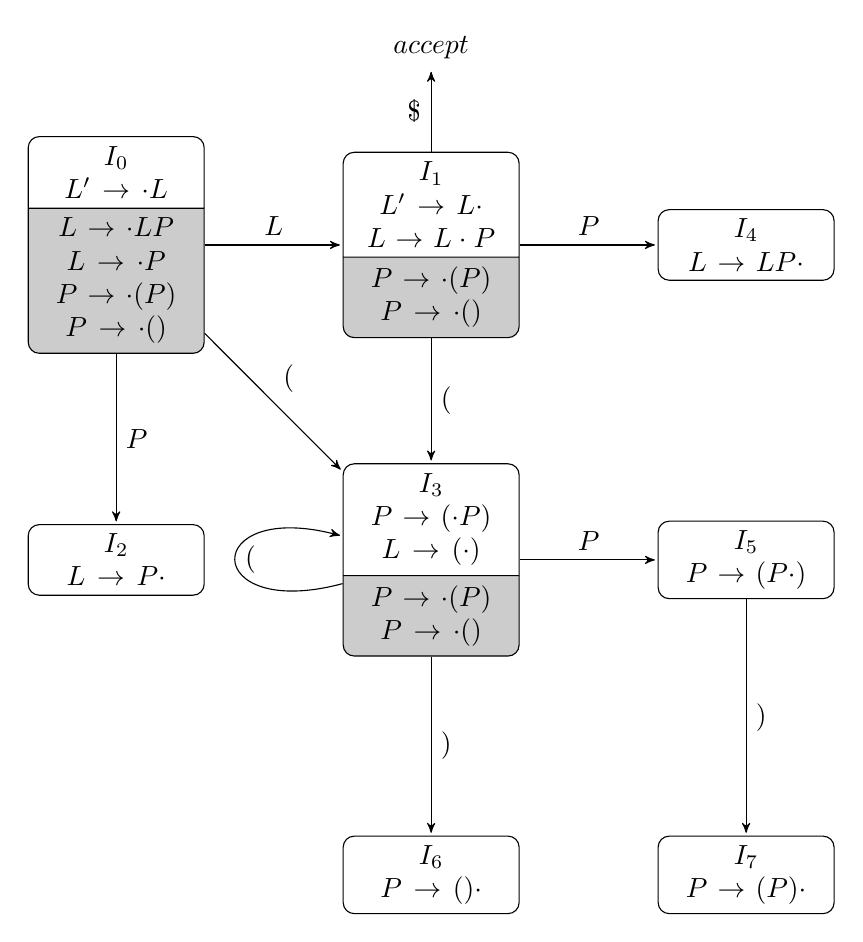
\begin{tikzpicture}[->,>=stealth',shorten >=1pt,node distance=4cm,on grid,scale = 1, auto]
    %% node
    % \draw [help lines] (0,0) grid (10,10); % 显示辅助格点位置
    \node (0) [draw,rounded corners, text centered, text width=2cm, 
    rectangle split, rectangle split parts=2,rectangle split part fill={white,gray!40} %Multi-part
        %anchor=north west, % node的锚点坐标,west为左边中央
      ]{
        $I_0$\\
        $L'\to \cdot L$
        \nodepart{two}
        $L\to \cdot LP$\\
        $L\to \cdot P$\\
        $P\to \cdot (P)$\\
        $P\to \cdot ()$
      }; % multi-part
    \node (1) [ right of=0,draw,rounded corners, text centered, text width=2cm, rectangle split, rectangle split parts=2,rectangle split part fill={white,gray!40}]
      {
        $I_1$\\
        $L'\to L \cdot$\\
        $L \to L \cdot P$
        \nodepart{two}
        $P\to \cdot (P)$\\
        $P\to \cdot ()$
      };
    \node (2) [below of=0,draw,rounded corners, text centered, text width=2cm]
      {
        $I_2$\\
        $L\to P \cdot$
      };  
    \node (3) [below  of=1,draw,rounded corners, text centered, text width=2cm, rectangle split, rectangle split parts=2,rectangle split part fill={white,gray!40}]
      {
        $I_3$\\
        $P\to ( \cdot P)$
        $L\to ( \cdot)$
        \nodepart{two}
        $P\to \cdot (P)$\\
        $P\to \cdot ()$
      };  
    \node (4) [right of=1,draw,rounded corners, text centered, text width=2cm]
      {
        $I_4$\\
        $L\to LP \cdot$
      };  
    \node (5) [right of=3,draw,rounded corners, text centered, text width=2cm]
      {
        $I_5$\\
        $P\to (P \cdot)$
      };   
    \node (6) [below of=3,draw,rounded corners, text centered, text width=2cm]
      {
        $I_6$\\
        $P\to ()\cdot$
      };   
    \node (7) [below of=5, draw,rounded corners, text centered, text width=2cm]
      {
        $I_7$\\
        $P\to (P)\cdot$
      };
    \node (8) [above of=1,yshift=-1.5cm]
      {
        $accept$
      };
    %% path
    \path (0) edge              node {$L$} (1)
      (0) edge              node {$P$} (2)
      (0) edge              node {$($} (3)
      (1) edge              node {$P$} (4)
      (1) edge              node {$($} (3)
      (3) edge              node {$P$} (5)
      (3) edge[loop left,right]   node {$($} (3)
      (3) edge              node {$)$} (6)
      (5) edge              node {$)$} (7)
      (1) edge              node {\$} (8);
    \end{tikzpicture} 

(3) \\
\indent\indent
\begin{tabular}{|c|c|c|c|c|c|}
  \hline
                           & \multicolumn{3}{c|}{ACTION}        & \multicolumn{2}{c|}{GOTO} \\ \hline
                           & (                       & )  & \$   & L           & P           \\ \hline
  0                        & \multicolumn{1}{r|}{s3} &    &     & g1          & g2          \\ \hline
  1                        & s3                      &    & accept &             & g4          \\ \hline
  2                        & r2                      & r2 & r2  &             &             \\ \hline
  3                        & s3                      & s6 &     &             & g5          \\ \hline
  4                        & r1                      & r1 & r1  &             &             \\ \hline
  5                        &                         & s7 &     &             &             \\ \hline
  6                        & r4                      & r4 & r4  &             &             \\ \hline
  7                        & r3                      & r3 & r3  &             &             \\ \hline
  \end{tabular}
  \\
  \indent\indent 该文法是$LR(0)$文法,因为$LR(0)$分析表没有冲突\\ 
(4) \\
\indent\indent
\begin{tabular}{|c|c|c|c|c|c|}
  \hline
                           & \multicolumn{3}{c|}{ACTION}        & \multicolumn{2}{c|}{GOTO} \\ \hline
                           & (                       & )  & \$   & L           & P           \\ \hline
  0                        & s3                      &    &     & g1          & g2          \\ \hline
  1                        & s3                      &    & accept &             & g4          \\ \hline
  2                        & r2                      &  & r2  &             &             \\ \hline
  3                        & s3                      & s6 &     &             & g5          \\ \hline
  4                        & r1                      &  & r1  &             &             \\ \hline
  5                        &                         & s7 &     &             &             \\ \hline
  6                        & r4                      & r4 & r4  &             &             \\ \hline
  7                        & r3                      & r3 & r3  &             &             \\ \hline
  \end{tabular}
  \\ \\
  \indent\indent \follow(L)=\{$(,\$ $\}, \follow(P)=\{$(,),\$ $\}\\
  \indent\indent 说明:按$X\to \gamma$规约时,当前分析的非终结符号$a$要满足:$a\in$\follow(X)\\
  \indent\indent 该文法是$SLR(1)$文法,因为$SLR(1)$分析表没有冲突\\ 
(4) \\
\indent 初始状态:0\\
\indent \textsc{PATH}:$0\to 3\to 3\to 6\to 5\to 7 \to 2\to 1\to 3 \to 6\to 4 \to 1\to accept$\\
\indent 用栈表示:$
  0\stackrel{\text{移入(}}{\longrightarrow} 03
  \stackrel{\text{移入(}}{\longrightarrow}  033
  \stackrel{\text{移入)}}{\longrightarrow}  0336
  \stackrel{\text{按4规约}}{\longrightarrow}  035
  \stackrel{\text{移入)}}{\longrightarrow}  0357
  \stackrel{\text{按3规约}}{\longrightarrow}  02
  \stackrel{\text{按2规约}}{\longrightarrow}  01
  \stackrel{\text{移入(}}{\longrightarrow}  013
  \stackrel{\text{移入)}}{\longrightarrow}  0136
  \stackrel{\text{按4规约}}{\longrightarrow}  014
  \stackrel{\text{按1规约}}{\longrightarrow}  01
  \to accept
  $
\end{solution}
%%%%%%%%%%%%%%%

%%%%%%%%%%%%%%%%%%%%
% 如果没有需要订正的题目,可以把这部分删掉

% \begincorrection
%%%%%%%%%%%%%%%%%%%%

%%%%%%%%%%%%%%%%%%%%
% 如果没有反馈,可以把这部分删掉
%%%%%%%%%%%%%%%%%%%%
\end{document}